This section focuses on the user interface point of view using UX UML diagram
to specify the possible interactions and the flow of events.
Layouts for the applications are described and outlined in section 3.1 of the
RASD.

\FloatBarrier
\begin{figure}
\centering
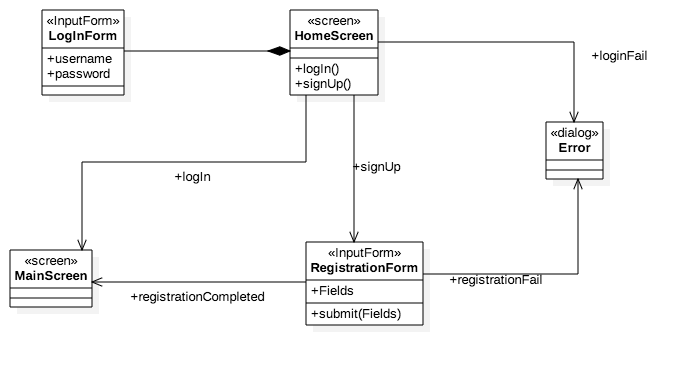
\includegraphics[scale=0.6]{Images/UID/u1.png}
\caption{User login screen}
\end{figure}
\FloatBarrier

\FloatBarrier
\begin{figure}
\centering
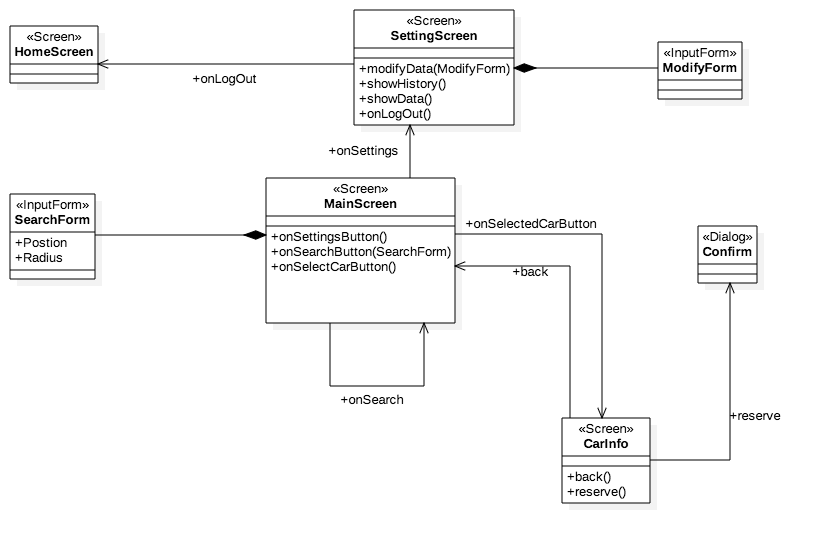
\includegraphics[scale=0.6]{Images/UID/u2.png}
\caption{User main screen}
\end{figure}
\FloatBarrier

\FloatBarrier
\begin{figure}
\centering
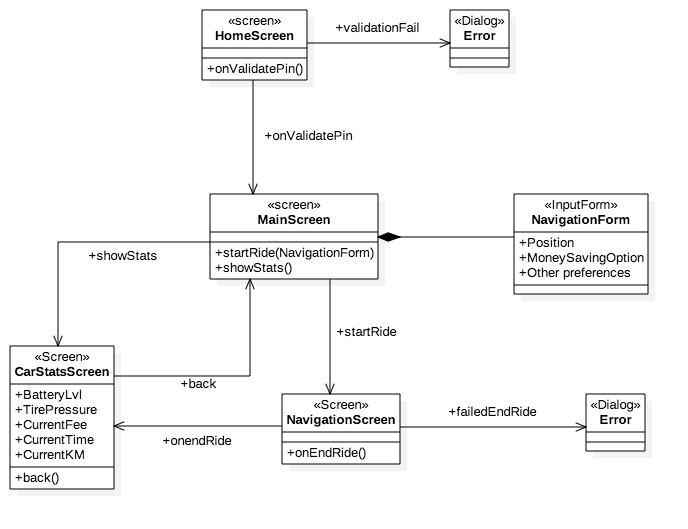
\includegraphics[scale=0.6]{Images/UID/u3.png}
\caption{Display screen flow}
\end{figure}
\FloatBarrier



